% Author: Seongjin Lee
% Hanyang University, Seoul, Korea
% esos.hanyang.ac.kr
% 2016-09-20
% note: some slides are adopted from  \url{www.cs.stevens.edu/~jschauma/631A/}
% https://github.com/resourceful/lecture_sysprog/

\documentclass[newPxFont,sthlmFooter,nooffset]{beamer}
\usepackage{kotex}
%\usetheme{sthlm}
\usepackage{../beamer_template/beamerthemesthlm}
\hypersetup{pdfauthor={Seongjin Lee (insight@gnu.ac.kr)},
            pdfsubject={Lecture Note: System Programming},
            pdfkeywords={Lecture Note, System Programming, class, (under)graduate},
            pdfmoddate={D: \pdfdate},
            pdfcreator={Seongjin Lee}}

%\setbeamertemplate{footline}[text line]{%
%    \parbox{\linewidth}{\vspace*{-8pt} \insertsectionhead  \hfill\insertshortauthor\hfill\insertpagenumber}}
%\setbeamertemplate{navigation symbols}{}




\title{System Programming}
\subtitle{Topic 8: Threads}
\author[SJL]{Seongjin Lee}
\institute{\href{mailto:insight@gnu.ac.kr}{insight@gnu.ac.kr}\\\url{http://open.gnu.ac.kr}\\Systems Research Lab.\\Gyeongsang National University}
\date{\today}

\begin{document}



\frame[plain]{\titlepage}

\frame[t]{\frametitle{Table of contents}\tableofcontents}


%---------------------------------------------------------



\begin{frame}[t]
  \frametitle{Introduction}

Limited amount of sharing can occur between related processes

\textit{thread of control} (or simply \textit{threads} to perform multiple tasks within the environment of a signle process.

All threads within a single process have access to the same process components, such as file descriptor and memory


  \begin{itemize}
  \item Threads Concepts
  \item Creation, Termination
  \item Consistency and synchronization mechanism
  \item Mutex, Reader-Writer Lock, Condition variable, Lock
  \end{itemize}

\end{frame}

\section{Thread Concepts}



\begin{frame}[t]
  \frametitle{Thread Concepts}
A typical UNIX process can be thought of as having a single thread of control:
\begin{itemize}
\item each process is doing only one thing at a time.
\end{itemize}

With multiple threads of control,
\begin{itemize}
\item we can design our programs to do more than one thing at a time
  within a single process,
\item each thread handles a separate task.
\end{itemize}


\end{frame}


\begin{frame}[t]
  \frametitle{Thread Concepts cnt'd}
There are several benefits
\begin{itemize}
\item We can simplify code that deals with asynchronous events by assigning a separate thread to handle each event type.
\item Threads automatically have access to the same memory address space and file descriptors.
\item  With multiple threads of control, the processing of independent tasks can be interleaved by assigning a separate thread per task.
\item  interactive programs can realize improved response time by using multiple threads to separate the portions of the program
\end{itemize}
\end{frame}



\begin{frame}[t]
  \frametitle{Thread Concepts cnt'd}
  Some people associate multithreaded programming with multiprocessor or multicore systems.
  \begin{itemize}
  \item The benefits of a multithreaded programming model can be
    realized even if your program is running on a uniprocessor.
  \item Some threads might be able to run while others are blocked
  \end{itemize}


\end{frame}



\begin{frame}[t]
  \frametitle{Thread Concepts cnt'd}
  A thread consists of the information necessary to represent an
    execution context within a process.
  \begin{itemize}
    \item  a thread ID that identifies the thread within a process,
    \item a set of register values,
    \item a stack,
    \item a scheduling priority and policy,
    \item a signal mask,
    \item an errno variable (recall Section 1.7),
    \item and thread-specific data (Section 12.6).
  \end{itemize}
Everything within a process is sharable among the threads in a process, including the text of the executable program, the program’s global and heap memory, the stacks, and the file descriptors

\end{frame}

\begin{frame}[fragile,t]
  \frametitle{Thread Identification}
  every thread has a thread ID
  \begin{itemize}
  \item thread ID has significance only within the context of the process to which it belongs.
  \end{itemize}

\bigskip
A thread ID is represented by the \texttt{pthread\_t} data type. Some times it is useful to print thread ID during program debugging

A thread can obtain its own thread ID by calling the \texttt{pthread\_self}
\begin{codedef}
#include <pthread.h>
int pthread_equal(pthread_t tid1, pthread_t tid2);
// Returns: nonzero if equal, 0 otherwise

pthread_t pthread_self(void);
Returns: the thread ID of the calling thre
\end{codedef}


\end{frame}


\begin{frame}[t]
  \frametitle{Thread Identification cnt'd}
  The master thread controls job assignment by placing the ID of the thread that should process the job in each job structure. Each worker thread then removes only jobs that are tagged with its own thread ID.

  \begin{figure}[h]
    \centering
    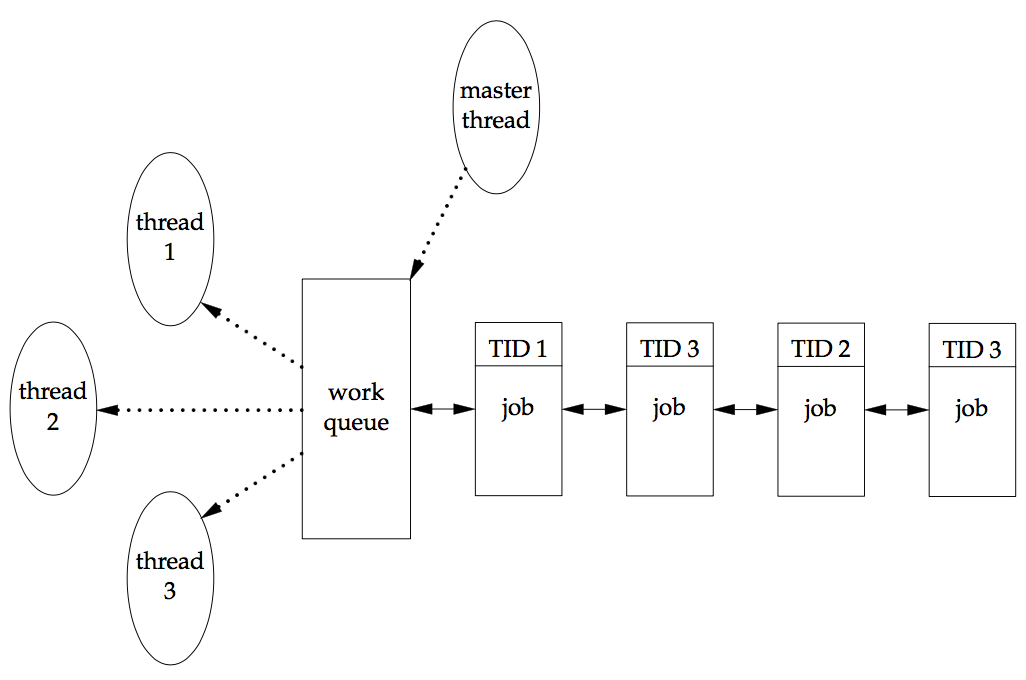
\includegraphics[width=0.7\linewidth]{figure/fig11-1}
    \caption{Work queue example}
    \label{fig:work}
  \end{figure}
\end{frame}


\section{Thread Creation and Termination}

\begin{frame}[fragile,t]
  \frametitle{Thread Creation}
  Additional threads can be created by calling the \texttt{pthread\_create}

  \begin{codedef}
#include <pthread.h>
int pthread_create(pthread_t *restrict tidp,
                   const pthread_attr_t *restrict attr,
                   void *(*start_rtn)(void *),
                   void *restrict arg);
// Returns: 0 if OK, error number on failure
  \end{codedef}

{\footnotesize
  \begin{itemize}
  \item The memory location pointed to by \textit{tidp} is set to the
    thread ID of the newly created thread
  \item \textit{attr} argument is used to customize various thread
    attributes.
  \item The newly created thread starts running at the address of the
    \textit{start\_rtn} function.
  \item This function takes a single argument, \textit{arg}, which is
    a typeless pointer.
  \item When a thread is created, there is no guarantee which will run
    first: the newly created thread or the calling thread.
  \item set of pending signals for the thread is cleared.
  \item Note that the pthread functions usually return an error code
    when they fail. They don’t set errno like the other POSIX
    functions.
  \end{itemize}
}
\end{frame}

\begin{frame}[fragile,t,allowframebreaks]
  \frametitle{Thread Creation: codes/print\_thrID.c}

\lstinputlisting[lineskip=0pt]{codes/print_thrID.c}

\begin{verbatim}
> ./print_thrID
main thread: pid 22813 tid 140736689316800 (0x7fffd05fa3c0)
new thread:  pid 22813 tid 123145322315776 (0x700001314000)
\end{verbatim}

\end{frame}

\begin{frame}[t]
  \frametitle{Thread Creation: codes/print\_thrID.c}

There are two oddities
\begin{itemize}
\item The first is the need to sleep in the main thread.
  \begin{itemize}
  \item If it doesn’t sleep, the main thread might exit, thereby
    terminating the entire process before the new thread gets a chance
    to run.
  \item This behavior is dependent on the operating system’s
    threads implementation and scheduling algorithms.
  \end{itemize}
\item The second oddity is that the new thread obtains its thread ID by calling \texttt{pthread\_self}
\end{itemize}

The main thread stores this ID in \texttt{ntid}, but the new thread can’t safely use it. If the new thread runs before the main thread returns from calling \texttt{pthread\_create}, then the new thread will see the uninitialized contents of \texttt{ntid} instead of the thread ID

\end{frame}


\begin{frame}[t]
  \frametitle{Thread Termination}
If any thread within a process calls \texttt{exit}, \texttt{\_Exit}, or \texttt{\_exit}, then the entire process terminates.

\uncover<2-> {A single thread can exit in three ways, thereby stopping its flow of control, without terminating the entire process.}
\begin{enumerate}
\item <2-> The thread can simply return from the start routine. The
  return value is the thread’s exit code.
\item <3-> The thread can be
  canceled by another thread in the same process.
\item  <4-> The thread can
  call \texttt{pthread\_exit}.
\end{enumerate}

\end{frame}


\begin{frame}[fragile, t]
  \frametitle{Thread Termination cnt'd}
 \texttt{pthread\_exit}
\begin{codedef}
#include <pthread.h>
void pthread_exit(void *rval_ptr);
\end{codedef}

{\footnotesize
 \begin{itemize}
 \item The \texttt{rval\_ptr} argument is a typeless pointer, similar
   to the single argument passed to the start routine.
 \item This pointer is
   available to other threads in the process by calling the
   \texttt{pthread\_join} function
 \item The calling thread will block until the specified thread calls \texttt{pthread\_exit}, returns from its start routine, or is canceled.
 \item If the thread simply returned from its start routine, \texttt{rval\_ptr} will contain the return code.
 \item If the thread was canceled, the memory location specified by \texttt{rval\_ptr} is set to \texttt{PTHREAD\_CANCELED}.
 \end{itemize}
}

\end{frame}

\begin{frame}[fragile, t]
  \frametitle{Thread Termination cnt'd}
 \texttt{pthread\_join}
\begin{codedef}
int pthread_join(pthread_t thread, void **rval_ptr);
// Returns: 0 if OK, error number on failure
\end{codedef}

{\footnotesize
 \begin{itemize}
 \item By calling \texttt{pthread\_join}, we automatically place the thread with which we’re joining in the detached state so that its resources can be recovered.
 \item If we are note interested in a thread's return value, we can set \texttt{rval\_ptr} to NULL
 \end{itemize}
}

\end{frame}



\begin{frame}[fragile,t,allowframebreaks]
  \frametitle{Thread Termination: codes/exit-state.c}

\lstinputlisting[lineskip=0pt]{codes/exit-state.c}

\begin{verbatim}
thread 1 returning
thread 2 exiting
thread 1 exit code 1
thread 2 exit code 2
\end{verbatim}

\end{frame}

\begin{frame}[t]
  \frametitle{Thread Termination cnt'd}
  \begin{itemize}
  \item The typeless pointer passed to \texttt{pthread\_create} and
    \texttt{pthread\_exit} can be used to pass more than a single
    value.
  \item Be careful that the memory used for the structure is still
    valid when the caller has completed.
  \item If a thread allocates a structure on its stack and passes a
    pointer to this structure to \texttt{pthread\_exit}, then the
    stack might be destroyed and its memory reused for something else
    by the time the caller of \texttt{pthread\_join} tries to use it.
  \end{itemize}

\end{frame}

\begin{frame}[fragile,t, allowframebreaks]
  \frametitle{Thread Termination cnt'd: exit-wrong.c}

\lstinputlisting[lineskip=0pt]{codes/exit-wrong.c}

\begin{verbatim}
./exit-wrong
thread 1:
  structure at 0x7000052d8ed0
  foo.a = 1
  foo.b = 2
  foo.c = 3
  foo.d = 4
parent starting second thread
thread 2: ID is 123145389182976
parent:
  structure at 0x7000052d8ed0
Segmentation fault: 11
\end{verbatim}

Even though the memory is still intact after the thread exits, we can’t depend on this always being the case. It certainly isn’t what we observe on the other platforms.
\end{frame}


\begin{frame}[fragile,t]
  \frametitle{Thread Termination cnt'd}
One thread can request that another in the same process be canceled by calling the \texttt{pthread\_cancel} function.

\begin{codedef}
#include <pthread.h>
int pthread_cancel(pthread_t tid);
// Returns: 0 if OK, error number on failure
\end{codedef}

In the default circumstances,
\begin{itemize}
\item \texttt{pthread\_cancel} will cause the thread specified by
  \textit{tid} to behave as if it had called \texttt{pthread\_exit}
  with an argument of \texttt{PTHREAD\_CANCELED}.
\end{itemize}

However, a thread can elect to ignore or otherwise control how it is canceled.
\begin{itemize}
\item it merely makes the request.
\end{itemize}

\end{frame}

\begin{frame}[t]
  \frametitle{Thread Termination cnt'd}
A thread can arrange for functions to be called when it exits, similar to the way as the \texttt{atexit} function

 The functions are known as \textit{thread cleanup handlers}.

More than one cleanup handler can be established for a thread.
\begin{itemize}
\item The handlers are recorded in a stack, which means that they are
  executed in the reverse order from that with which they were
  registered.
\end{itemize}

\end{frame}


\begin{frame}[fragile,t]
  \frametitle{Thread Termination cnt'd}
\begin{codedef}
#include <pthread.h>
void pthread_cleanup_push(void (*rtn)(void *), void *arg);
void pthread_cleanup_pop(int execute};
\end{codedef}

The \texttt{pthread\_cleanup\_push} function schedules the cleanup function, \textit{rtn}, to be called with the single argument, \textit{arg}, when the thread performs one of the following actions:
\begin{enumerate}
\item Makes a call to \texttt{pthread\_exit}
\item Responds to a cancellation request
\item Makes a call to \texttt{pthread\_cleanup\_pop} with a nonzero
  execute argument
\end{enumerate}

\end{frame}

\begin{frame}[fragile,t]
  \frametitle{Thread Termination cnt'd}
\begin{codedef}
#include <pthread.h>
void pthread_cleanup_push(void (*rtn)(void *), void *arg);
void pthread_cleanup_pop(int execute};
\end{codedef}

If the \textit{execute} argument is set to zero, the cleanup function is not called.
\begin{itemize}
\item In either case, \texttt{pthread\_cleanup\_pop} removes the
  cleanup handler established by the last call to
  \texttt{pthread\_cleanup\_push}.
\end{itemize}

They can be used as macros
\end{frame}


\begin{frame}[fragile,t, allowframebreaks]
  \frametitle{Thread Termination cnt'd: codes/push-pop.c }

\lstinputlisting[lineskip=0pt]{codes/push-pop.c}


\begin{verbatim}
./push-pop
thread 1 start
thread 2 start
thread 1 push complete
thread 2 push complete
cleanup: thread 1 second handler
cleanup: thread 2 second handler
cleanup: thread 2 first handler
Segmentation fault: 11
\end{verbatim}
\end{frame}


\begin{frame}[t]
  \frametitle{Thread Termination cnt'd}

  \begin{figure}[h]
    \centering
    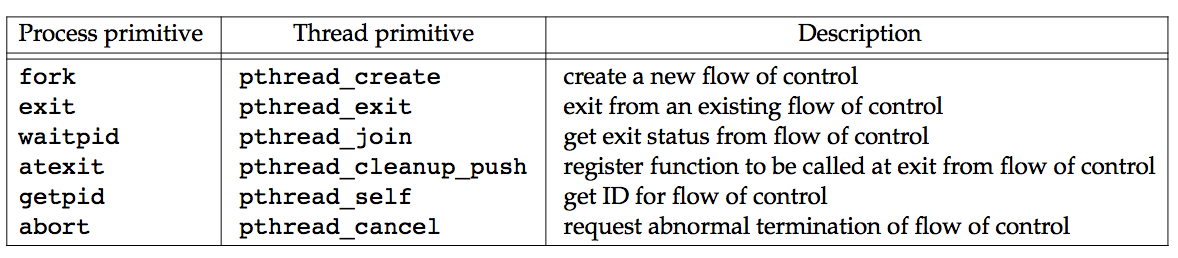
\includegraphics[width=\linewidth]{figure/fig11-6}
    \caption{Comparison of process and thread primitives}
    \label{fig:work}
  \end{figure}

By default thread’s termination status is retained until we call \texttt{pthread\_join} for that thread.


\end{frame}

\begin{frame}[t,fragile]
  \frametitle{Thread Termination cnt'd}
  A thread’s underlying storage can be reclaimed immediately on termination if the thread has been detached.
  \begin{codedef}
#include <pthread.h>
int pthread_detach(pthread_t tid);
//Returns: 0 if OK, error number on failure
  \end{codedef}

we can create a thread that is already in the detached state by modifying the thread attributes we pass to \texttt{pthread\_create}.

\end{frame}



\section{Thread Synchronization}
\begin{frame}[t]
  \frametitle{Thread Synchronization}
we need to make sure that each thread sees a consistent view of its data.

when one thread can modify a variable that other threads can read or
modify
\begin{itemize}
\item we need to synchronize the threads to ensure that
  they don’t use an invalid value when accessing the variable’s memory
  contents.
\end{itemize}
When one thread modifies a variable, other threads can
  potentially see inconsistencies when reading the value of that  variable.

\end{frame}

\begin{frame}[t]
  \frametitle{Thread Synchronization cnt'd}
thread A reads the variable and then writes a new value to
  it, but the write operation takes two memory cycles.

If thread B reads the same variable between the two write cycles, it will see an inconsistent value.

  \begin{figure}[h]
    \centering
    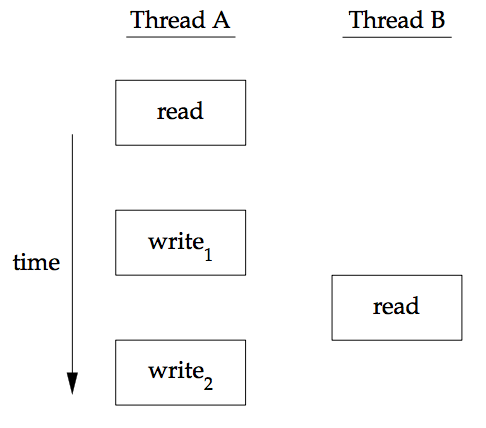
\includegraphics[width=0.4\linewidth]{figure/fig11-7}
    \caption{Interleaved memory cycles with two threads}
    \label{fig:work}
  \end{figure}


\end{frame}



\begin{frame}[t]
  \frametitle{Thread Synchronization cnt'd}
To solve this problem, the threads have to use a lock that will allow only one thread to access the variable at a time.

  \begin{figure}[h]
    \centering
    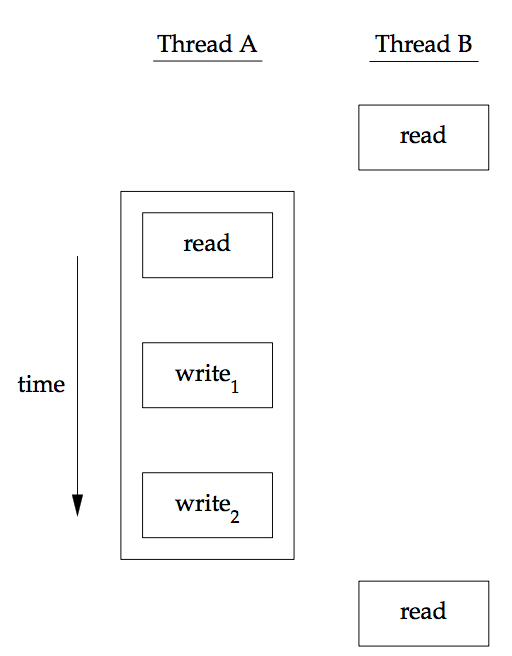
\includegraphics[width=0.4\linewidth]{figure/fig11-8}
    \caption{Two threads synchronizing memory access}
    \label{fig:work}
  \end{figure}


\end{frame}




\begin{frame}[t]
  \frametitle{Thread Synchronization cnt'd}
We also need to synchronize two or more threads that might try to modify the same variable at the same time.

The increment operation is usually broken down into three steps.
\begin{enumerate}
\item  Read the memory location into a register.
\item  Increment the value in the register.
\item  Write the new value back to the memory location
\end{enumerate}

If two threads try to increment the same variable at almost the same time without synchronizing with each other, the results can be inconsistent.

If the modification is atomic, then there isn’t a race.

\end{frame}



\begin{frame}[t]
  \frametitle{Thread Synchronization cnt'd}

  \begin{figure}[h]
    \centering
    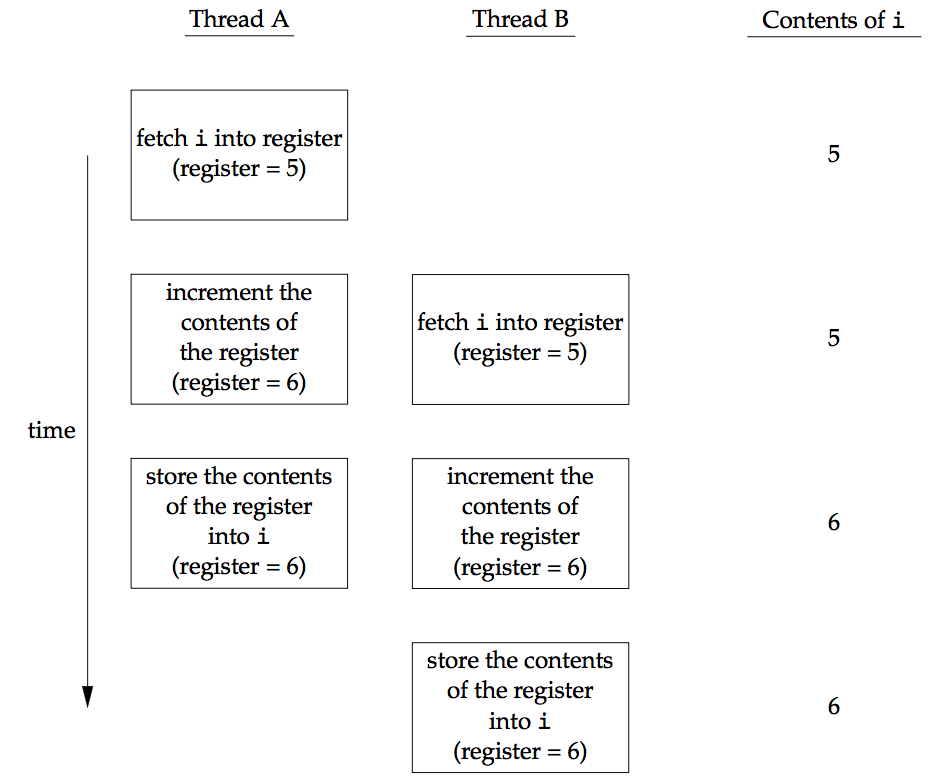
\includegraphics[width=0.7\linewidth]{figure/fig11-9}
    \caption{Two unsynchronized threads incrementing the same variable}
    \label{fig:work}
  \end{figure}


\end{frame}




\subsection{Mutexes}

\begin{frame}[t]
  \frametitle{Mutexes}
  We can protect our data and ensure access by only one thread at a time by using the pthreads mutual-exclusion interfaces.

A mutex is basically a lock
\begin{itemize}
\item we set (lock) before accessing a shared resource and release (unlock) when we’re done.
\item While it is set, any other thread that tries to set it will block until we release it.
\item If more than one thread is blocked when we unlock the mutex,
  \begin{itemize}
  \item then all threads blocked on the lock will be made runnable,
  \item and the first one to run will be able to set the lock.
  \end{itemize}
\item The others will see that the mutex is still locked and go back to waiting for it to become available again.
\end{itemize}

\end{frame}


\begin{frame}[t]
  \frametitle{Mutexes cnt'd}
Mutual-exclusion mechanism works only if we design our threads to follow the same data-access rules.
\begin{itemize}
\item The operating system doesn’t serialize access to data for us.
\end{itemize}

If we allow one thread to access a shared resource without first
  acquiring a lock
  \begin{itemize}
  \item then inconsistencies can occur even though the rest of our
    threads do acquire the lock before attempting to access the shared
    resource
  \end{itemize}
\end{frame}


\begin{frame}[fragile,t]
  \frametitle{Mutexes cnt'd}
A mutex variable is represented by the \texttt{pthread\_mutex\_t} data type.

We must first initialize it by either
\begin{itemize}
\item setting it to the constant \texttt{PTHREAD\_MUTEX\_INITIALIZER}
  (for statically allocated mutexes only)
\item or calling \texttt{pthread\_mutex\_init}.
\end{itemize}

If we allocate the mutex dynamically (by calling malloc, for example),
then we need to call \texttt{pthread\_mutex\_destroy} before freeing the memory.

\begin{codedef}
#include <pthread.h>
int pthread_mutex_init(pthread_mutex_t *restrict mutex,
                       const pthread_mutexattr_t *restrict attr);
int pthread_mutex_destroy(pthread_mutex_t *mutex);
//Both return: 0 if OK, error number on failure
\end{codedef}

To initialize a mutex with the default attributes, we set \textit{attr} to \texttt{NULL}
\end{frame}


\begin{frame}[fragile,t]
  \frametitle{Mutexes cnt'd}
To lock a mutex, we call \texttt{pthread\_mutex\_lock}.

If the mutex is already locked,
\begin{itemize}
\item the calling thread will block until the mutex is unlocked.
\end{itemize}
To unlock a mutex, we call \texttt{pthread\_mutex\_unlock}.
\begin{codedef}
#include <pthread.h>
int pthread_mutex_lock(pthread_mutex_t *mutex);
int pthread_mutex_trylock(pthread_mutex_t *mutex);
int pthread_mutex_unlock(pthread_mutex_t *mutex);
// All return: 0 if OK, error number on failure
\end{codedef}
If a thread can’t afford to block, it can use \texttt{pthread\_mutex\_trylock} to lock the mutex conditionally

\end{frame}

\begin{frame}[fragile,t, allowframebreaks]
  \frametitle{Mutexes cnt'd: \texttt{codes/mutex1.c}}
Following example illustrates a mutex used to protect a data structure.

When more than one thread needs to access a dynamically allocated object, we can embed a reference count in the object to ensure that we don’t free its memory before all threads are done using it

\lstinputlisting[lineskip=0pt]{codes/mutex1.c}

No locking is necessary necessary when we initialize the reference count to 1 in the \texttt{foo\_alloc} function, because the allocating thread is the only reference to it so far.

In this example, we have ignored how threads find an object before calling \texttt{foo\_hold}.

Even though the reference count is zero, it would be a mistake for \texttt{foo\_rele} to free the object’s memory if another thread is blocked on the mutex in a call to \texttt{foo\_hold}.
\end{frame}








\subsection{Deadlock Avoidance}
\begin{frame}[t]
  \frametitle{Deadlock Avoidance}
when we use more than one mutex in our programs, a deadlock can occur
\begin{itemize}
\item  if we allow one thread to hold a mutex and
  block while trying to lock a second mutex at the same time that
  another thread holding the second mutex tries to lock the first
  mutex.
\end{itemize}
Deadlocks can be avoided by carefully controlling the order in which mutexes are locked.
\begin{itemize}
\item If all threads always lock mutex A before mutex B, no deadlock can occur from the use of the two mutexes
\end{itemize}

Sometimes, an application’s architecture makes it difficult to apply a lock ordering
\end{frame}


\begin{frame}[fragile,t, allowframebreaks]
  \frametitle{Deadlock Avoidance cnt'd: \texttt{codes/mutex2.c}}
In this example, we use two mutexes to avoid dealocks by always lock them in the same order

The second mutex protects a hash list that we use to keep track of the foo data structure

\texttt{hashlock} mutex protects both the \texttt{fh} hash table and the \texttt{f\_next} hash link field in the \texttt{foo} structure. The \texttt{f\_lockmutex} in the \texttt{foo} structure protects access to the remainder of the foo structure’s fields.

\lstinputlisting[lineskip=0pt]{codes/mutex2.c}


\end{frame}

\begin{frame}[fragile,t, allowframebreaks]
  \frametitle{Deadlock Avoidance cnt'd: \texttt{codes/mutex3.c}}
This locking approach is complex, so we need to revisit our design.

We can simplify things considerably by using the hash list lock to protect the structure reference count, too.

The structure mutex can be used to protect everything else in the foo structure.
\lstinputlisting[lineskip=0pt]{codes/mutex3.c}

\end{frame}

\begin{frame}[t]
  \frametitle{Deadlock Avoidance cnt'd}
If your locking granularity is too coarse,
\begin{itemize}
\item you end up with too many threads blocking behind the same locks,
  with little improvement possible from concurrency.
\end{itemize}
If your locking granularity is too fine,
\begin{itemize}
\item then you suffer bad performance from excess locking overhead,
  and you end up with complex code.
\end{itemize}

\end{frame}

\begin{frame}[fragile, t]
  \frametitle{Deadlock Avoidance cnt'd}
One additional mutex primitive allows us to bound the time that a thread blocks when a mutex it is trying to acquire is already locked.

The \texttt{pthread\_mutex\_timedlock} function is equivalent to \texttt{pthread\_mutex\_lock},
\begin{itemize}
\item but if the timeout value is reached, \texttt{pthread\_mutex\_timedlock}
\end{itemize}

\begin{codedef}
#include <pthread.h>
#include <time.h>
int pthread_mutex_timedlock(pthread_mutex_t *restrict mutex,
                           const struct timespec *restrict tsptr);
// Returns: 0 if OK, error number on failure
\end{codedef}
\end{frame}

\begin{frame}[fragile, t,allowframebreaks]
  \frametitle{\texttt{pthread\_mutex\_timedlock} Fuction: \texttt{codes/timedlock.c}}
how to use \texttt{pthread\_mutex\_timedlock} to avoid blocking indefinitely.

note that Mac OS does not have \texttt{pthread\_mutex\_timedlock}
\lstinputlisting[lineskip=0pt]{codes/timedlock.c}

This program deliberately locks a mutex it already owns to demonstrate how \texttt{pthread\_mutex\_timedlock} works. This strategy is not recommended in practice, because it can lead to deadlock.
\end{frame}

\subsection{Reader-Writer Locks}


\begin{frame}[t]
  \frametitle{Reader-Writer Locks}
Reader–writer locks are similar to mutexes, except that they allow for higher degrees of parallelism.

Three states are possible with a reader–writer lock:
\begin{enumerate}
\item locked in read mode,
\item locked in write mode,
\item and unlocked.
\end{enumerate}

Only one thread at a time can hold a reader–writer lock in write mode,
\begin{itemize}
\item but multiple threads can hold a reader–writer lock in read mode
  at the same time.
\end{itemize}

\end{frame}

\begin{frame}[t]
  \frametitle{Reader-Writer Locks cnt'd}
When a reader–writer lock is write locked,
\begin{itemize}
\item all threads attempting to lock it block until it is unlocked.
\end{itemize}
When a reader–writer lock is read locked,
\begin{itemize}
\item all threads attempting to lock it in read mode are given access,
\item but any threads attempting to lock it in write mode block until all
  the threads have released their read locks.
\end{itemize}

Reader–writer locks are well suited for situations in which data structures are read more often than they are modified.

Reader–writer locks are also called shared–exclusive locks.
\end{frame}


\begin{frame}[t,fragile]
  \frametitle{Reader-Writer Locks cnt'd}
eader–writer locks must be initialized before use and destroyed before freeing their underlying memory.

\begin{codedef}
#include <pthread.h>
int pthread_rwlock_init(pthread_rwlock_t *restrict rwlock,
                        const pthread_rwlockattr_t *restrict attr);
int pthread_rwlock_destroy(pthread_rwlock_t *rwlock);
// Both return: 0 if OK, error number on failure
\end{codedef}
A reader–writer lock is initialized by calling \texttt{pthread\_rwlock\_init}.

Before freeing the memory backing a reader–writer lock, we need to call \texttt{pthread\_rwlock\_destroy} to clean it up.
\end{frame}


\begin{frame}[t, fragile]
  \frametitle{Reader-Writer Locks cnt'd}
To lock a reader–writer lock in read mode, we call \texttt{pthread\_rwlock\_rdlock}.

To write lock a reader–writer lock, we call \texttt{pthread\_rwlock\_wrlock}.

Regardless of how we lock a reader–writer lock, we can unlock it by calling \texttt{pthread\_rwlock\_unlock}.

\begin{codedef}
#include <pthread.h>
int pthread_rwlock_rdlock(pthread_rwlock_t *rwlock);
int pthread_rwlock_wrlock(pthread_rwlock_t *rwlock);
int pthread_rwlock_unlock(pthread_rwlock_t *rwlock);
// All return: 0 if OK, error number on failure
\end{codedef}
\end{frame}


\begin{frame}[t,fragile, allowframebreaks]
  \frametitle{Reader-Writer Locks cnt'd: \texttt{codes/rwlock.c}}
use of reader–writer lock

A queue of job requests is protected by a single reader–writer lock.

\lstinputlisting[lineskip=0pt]{codes/rwlock.c}
\end{frame}



\subsection{Condition Variables}

\begin{frame}[t]
  \frametitle{Condition Variables}
Condition variables are another synchronization mechanism available to threads.
\begin{itemize}
\item When used with mutexes, condition variables allow threads to
  wait in a race-free way for arbitrary conditions to occur.
\end{itemize}

The condition itself is protected by a mutex.
\begin{itemize}
\item A thread must first lock the mutex to change the condition
  state.
\item Other threads will not notice the change until they acquire
  the mutex,
\item because the mutex must be locked to be able to evaluate
  the condition.
\end{itemize}

\end{frame}



\begin{frame}[t, fragile]
  \frametitle{Condition Variables cnt'd}
Before a condition variable is used, it must first be initialized.

A condition variable, represented by the \texttt{pthread\_cond\_t} data type, can be initialized in two ways.
\begin{itemize}
\item We can assign the constant \texttt{PTHREAD\_COND\_INITIALIZER} to a
  statically allocated condition variable,
\item if the condition variable is allocated dynamically, we can use
  the \texttt{pthread\_cond\_init} function to initialize it.
\end{itemize}

We can use the \texttt{pthread\_cond\_destroy} function to deinitialize a condition variable before freeing its underlying memory.

\begin{codedef}
#include <pthread.h>
int pthread_cond_init(pthread_cond_t *restrict cond,
                      const pthread_condattr_t *restrict attr);
int pthread_cond_destroy(pthread_cond_t *cond);
// Both return: 0 if OK, error number on fa
\end{codedef}

\end{frame}



\begin{frame}[t, fragile]
  \frametitle{Condition Variables cnt'd}
\texttt{pthread\_cond\_wait} to wait for a condition to be true

\begin{codedef}
#include <pthread.h>
int pthread_cond_wait(pthread_cond_t *restrict cond,
                      pthread_mutex_t *restrict mutex);
int pthread_cond_timedwait(pthread_cond_t *restrict cond,
                      pthread_mutex_t *restrict mutex,
                      const struct timespec *restrict tsptr);
// Both return: 0 if OK, error number on failure
\end{codedef}

The mutex passed to \texttt{pthread\_cond\_wait} protects the condition.

The caller passes it locked to the function, which then atomically places the calling thread on the list of threads waiting for the condition and unlocks the mutex.

 When \texttt{pthread\_cond\_wait} returns, the mutex is again locked.
\end{frame}

\begin{frame}[t, fragile]
  \frametitle{Condition Variables cnt'd}
There are two functions to notify threads that a condition has been satisfied.
\begin{itemize}
\item The \texttt{pthread\_cond\_signal} function will wake up at least one
  thread waiting on a condition,
\item whereas the \texttt{pthread\_cond\_broadcast} function will wake
  up all threads waiting on a condition.
\end{itemize}

\begin{codedef}
#include <pthread.h>
int pthread_cond_signal(pthread_cond_t *cond);
int pthread_cond_broadcast(pthread_cond_t *cond);
// Both return: 0 if OK, error number on f
\end{codedef}
When we call \texttt{pthread\_cond\_signal} or \texttt{pthread\_cond\_broadcast}, we are said to be signaling the thread or condition. We have to be careful to signal the threads only after changing the state of the condition.
\end{frame}

\begin{frame}[t, fragile, allowframebreaks]
  \frametitle{Condition Variables cnt'd: \texttt{codes/condvar.c}}
example of how to use a condition variable and a mutex together to synchronize threads.
\lstinputlisting[lineskip=0pt]{codes/condvar.c}

We protect the condition with a mutex and evaluate the condition in a while loop.
\begin{itemize}
\item When we put a message on the work queue, we need to hold the
  mutex,
\item but we don’t need to hold the mutex when we signal the
  waiting threads.
\end{itemize}

Since we check the condition in a while loop, this doesn’t present a problem;
\begin{itemize}
\item a thread will wake up, find that the queue is still empty, and
  go back to waiting again.
\end{itemize}

\end{frame}

\subsection{Spin Locks}

\begin{frame}[t]
  \frametitle{Spin Locks}
A spin lock is like a mutex,
\begin{itemize}
\item process is blocked by busy-waiting (spinning) until the lock can be acquired
\end{itemize}
A spin lock could be used in situations where locks are held for short periods of times and threads don’t want to incur the cost of being descheduled.

\end{frame}

\begin{frame}[t]
  \frametitle{Spin Locks cnt'd}
Spin locks are often used as low-level primitives to implement other types of locks.

while a thread is spinning and waiting for a lock to become available, the CPU can’t do anything else.
\end{frame}


\begin{frame}[t, fragile]
  \frametitle{Spin Locks cnt'd}
We can initialize a spin lock with the \texttt{pthread\_spin\_init} function.

To deinitialize a spin lock, we can call the \texttt{pthread\_spin\_destroy} function.

\begin{codedef}
#include <pthread.h>
int pthread_spin_init(pthread_spinlock_t *lock, int pshared);
int pthread_spin_destroy(pthread_spinlock_t *lock);
// Both return: 0 if OK, error number on fai
\end{codedef}

The \textit{pshared} argument represents the process-shared attribute, which indicates how the spin lock will be acquired
\begin{itemize}
\item \texttt{PTHREAD\_PROCESS\_SHARED} - shared among processes
\item  \texttt{PTHREAD\_PROCESS\_PRIVATE} - shared within processes
\end{itemize}
\end{frame}

\begin{frame}[t, fragile]
  \frametitle{Spin Locks cnt'd}

To lock the spin lock,
\begin{itemize}
\item we can call either \texttt{pthread\_spin\_lock}, which will spin
  until the lock is acquired,
\item or \texttt{pthread\_spin\_trylock}, which will return the
  \texttt{EBUSY} error if the lock can’t be acquired immediately.
\end{itemize}

  \begin{codedef}
#include <pthread.h>
int pthread_spin_lock(pthread_spinlock_t *lock);
int pthread_spin_trylock(pthread_spinlock_t *lock);
int pthread_spin_unlock(pthread_spinlock_t *lock);
All return: 0 if OK, error number on failure
  \end{codedef}

Note that if a spin lock is currently unlocked,
\begin{itemize}
\item then the \texttt{pthread\_spin\_lock} function can lock it without
  spinning.
\item If the thread already has it locked or unlocked, the results are undefined.
\end{itemize}

\end{frame}

\subsection{Barriers}
\begin{frame}[t]
  \frametitle{Barriers}
Barriers are a synchronization mechanism that can be used to coordinate multiple threads working in parallel.
\begin{itemize}
\item A barrier allows each thread to wait until all cooperating
  threads have reached the same point, and then continue executing
  from there.
\item the \texttt{pthread\_join} function acts as a barrier to allow
  one thread to wait until another thread exits.
\end{itemize}
They allow an arbitrary number of threads to wait until all of the threads have completed processing,
\begin{itemize}
\item but the threads don’t have to exit.
\item They can continue working after all threads have reached the
  barrier.
\end{itemize}

\end{frame}

\begin{frame}[t, fragile]
  \frametitle{Barriers cnt'd}
We can use the \texttt{pthread\_barrier\_init} function to initialize a barrier,

we can use the \texttt{pthread\_barrier\_destroy} function to deinitialize a barrier.
\begin{codedef}
#include <pthread.h>
int pthread_barrier_init(pthread_barrier_t *restrict barrier,
                         const pthread_barrierattr_t *restrict attr,
                         unsigned int count);
int pthread_barrier_destroy(pthread_barrier_t *barrier);
// Both return: 0 if OK, error number on failure
\end{codedef}

\begin{itemize}
\item \textit{count} argument to specify the number of threads that must reach the barrier before all of the threads will be allowed to continue.
\item \textit{attr} argument to specify the attributes of the barrier object
(\textit{attr} to NULL = default)
\item resoureces initialized with \texttt{pthread\_barrier\_init} must be deinitialized with \texttt{pthread\_barrier\_destroy}
\end{itemize}

\end{frame}


\begin{frame}[t, fragile]
  \frametitle{Barriers cnt'd}
We use the \texttt{pthread\_barrier\_wait} function to indicate that a thread is done with its work and is ready to wait for all the other threads to catch up.
\begin{codedef}
#include <pthread.h>
int pthread_barrier_wait(pthread_barrier_t *barrier);
// Returns: 0 or PTHREAD_BARRIER_SERIAL_THREAD if OK, error number on failure
\end{codedef}
The thread calling \texttt{pthread\_barrier\_wait} is put to sleep
\begin{itemize}
\item if the barrier count (set in the call to \texttt{pthread\_barrier\_init})
  is not yet satisfied.
\item If the thread is the last one to \texttt{call pthread\_barrier\_wait}, thereby satisfying the barrier count, all of the threads are awakened.
\item Once the barrier count is reached and the threads are unblocked, the barrier can be used again. The count can't be changed
\end{itemize}

\end{frame}


\begin{frame}[t, fragile, allowframebreaks]
  \frametitle{Barriers cnt'd: \texttt{code/barrier.c}}

note that mac OS does not have \texttt{pthread\_barrier\_wait}
\lstinputlisting[lineskip=0pt]{codes/barrier.c}

\end{frame}


\begin{frame}[t]
  \frametitle{Barriers cnt'd}

\end{frame}





\begin{comment}
%---------------------------------------------------------
\section{Last Words}

\begin{frame}[t]
  \frametitle{Last Words}

\begin{itemize}
\item Read Chapter 12
\end{itemize}
\end{frame}
\end{comment}

\end{document}
